\subsection{Test setup}

Our program was written in C/C++ and compiled with Clang. All memory allocations were cache line boundary aligned.

All benchmarks were performed on a Linux desktop which has 4 GB ram and a Core i3 550 CPU with the following specification:

\begin{itemize}
\item 2 * 3.2 GHz (no Turbo boost)
\item 2 * 32 KB L1 instruction cache
\item 2 * 32 KB L1 data cache
\item 2 * 256 KB L2 cache
\item Shared 4 MB L3 cache
\item 64 byte cache lines
\item Inclusive caches
\item The associativity for the cache levels are 8, 8 and 16 respectively
% http://www.ni.com/white-paper/11266/en#toc5
\item Disabled adjacent cache line prefetcher
\end{itemize}

Initially, we measured L1 cache faults, L2 cache faults, branch predictions etc. using PAPI. However, we got results we found ridiculously high.
For instance, we got 79 L2 cache faults for each binary search query where each query used 24 iterations.
We would expect at most 24 L2 cache faults per query. And 24 cache faults should only occur when the cache is cold.

Consequently, we tried Intel's PAPI equivalent Intel Performance Counters Monitor (IPCM) and got a more sane 15 cache faults.
That is still above what we expect according to the previously derived formulas but Core i3 use prefetchers and our formulas does not take associativity into account which could affect the number.

We eventually settled on using as much data from IPCM as possible because they seemed more realistic and because we
assume Intel knowns more about their hardware than third-parties does. However, IPCM is not capable of measuring branch mispredictions. So for that we used PAPI.

Comparison counts were measured with counting integrated into the source code. These counters were removed when running time was measured. The running time was wall time.

\todo{Preprocessing er ikke talt med}

All tests were performed 5 times and the median was selected. For each
test we ran 10,000,000 queries. The data were randomly generated with
an uniform distribution. The range of the data was MIN\_INT to
MAX\_INT - 1. As mentioned, the max value is MAX\_INT - 1 and not
MAX\_INT, because MAX\_INT is used as dummy data. Queries were also
randomly generated with the same distribution. Therefore, we were able
to make the assumption that the top of the tree is in cache after some
number of queries. In contrast, if the queries are sorted then for
each query we would have the entire path or almost the entire path in
cache. And we would get a linear number of cache faults in total.

\subsection{Binary Search}
From the RAM model, we would expect the query time normalized with the
logarithm of the input size, to be a
constant. Figure~\ref{fig:bs_runningtime} clearly shows that this is
not what we are experiencing when running the binary search algorithm on our
test setup.

\begin{figure}[h!]
  \centering
  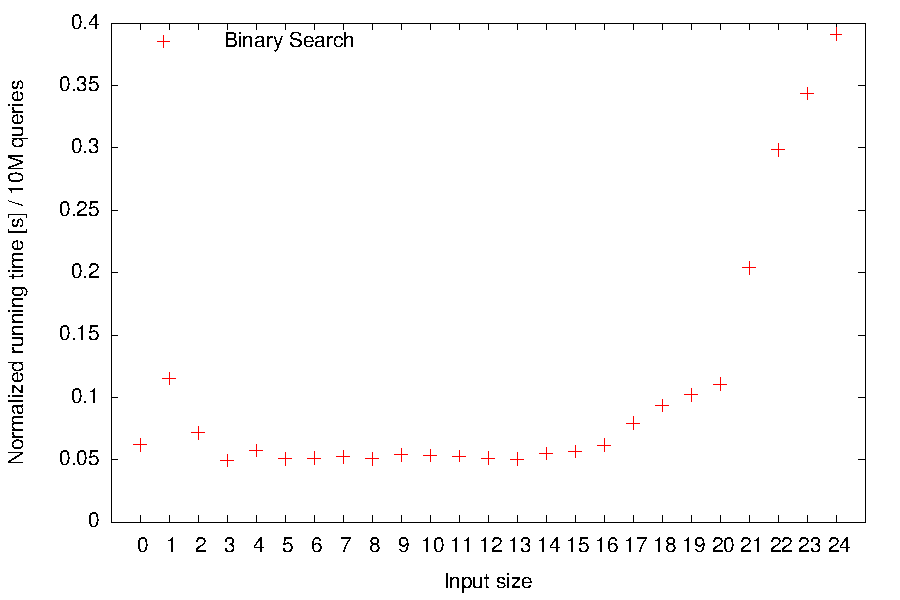
\includegraphics[width=\textwidth]{../week1/plots/outputs/bs_runningtime}
  \caption{Normalized time to perform 10 million queries. The input
    size axis is the base-2 logarithm to the input size.}
  \label{fig:bs_runningtime}
\end{figure}

From figure~\ref{fig:bs_runningtime} we see the first small increase
at input size \(2^{13}\), a somewhat larger increase at \(2^{16}\),
and it behaves very badly with more than \(2^{20}\) elements.
These numbers corresponds to the CPU's L1, L2 and L3 cache sizes. We
therefore suspect cache faults to be the
bottleneck. Figure~\ref{fig:bs_cachefaults} shows the number of cache
faults per query. It clearly shows that there is a correlation between cache faults and the time to execute a query.

\begin{figure}[h!]
  \centering
  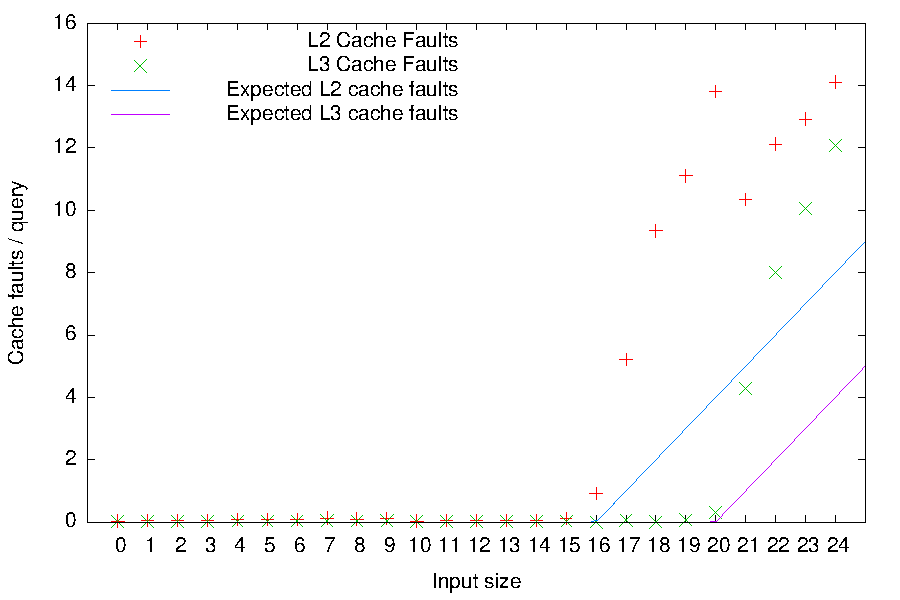
\includegraphics[width=\textwidth]{../week1/plots/outputs/bs_cachefaults}
  \caption{Cache faults measured per query and the expected number of cache faults.}
  \label{fig:bs_cachefaults}
\end{figure}

Figure~\ref{fig:bs_cachefaults} shows that we get even more cache
faults than we expect. We think this may be explained by cache
associativity\todo{Should we detail our explanation of this?}.

\subsection{BFS and DFS layout}
In order to improve the query time for large inputs, we try to
reduce the number of cache faults. We expect a better cache
performance using a BFS or DFS memory
layout. Figure~\ref{fig:bfs_dfs_runningtime} shows the query times of
such layouts.
\begin{figure}[h!]
  \centering
  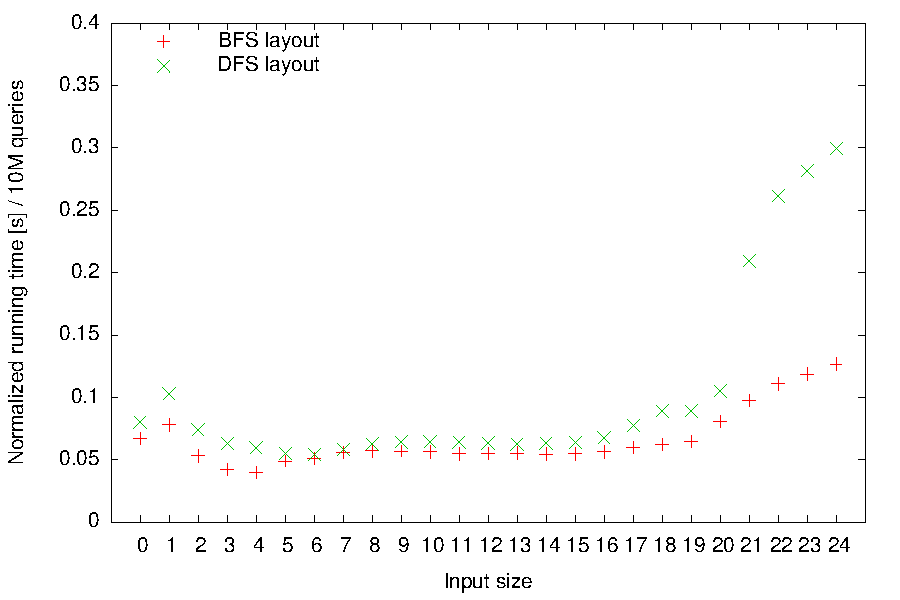
\includegraphics[width=\textwidth]{../week1/plots/outputs/bfs_dfs_runningtime}
  \caption{Normalized query time using BFS/DFS layouts.}
  \label{fig:bfs_dfs_runningtime}
\end{figure}
Both these layouts performs better than the in-order binary search,
but the DFS layout seems to perform worse than the BFS layout. This is quite unexpected as we expect fewer cache faults. The amount of cache faults is shown in figure~\ref{fig:bfs_dfs_cachefaults}. This plot is even more surprising. The cache faults for BFS and DFS is reversed compared to our expectations.

We do not have a satisfactory explanation for these results. Cache associativity might play a role.


\begin{figure}[h!]
  \centering
  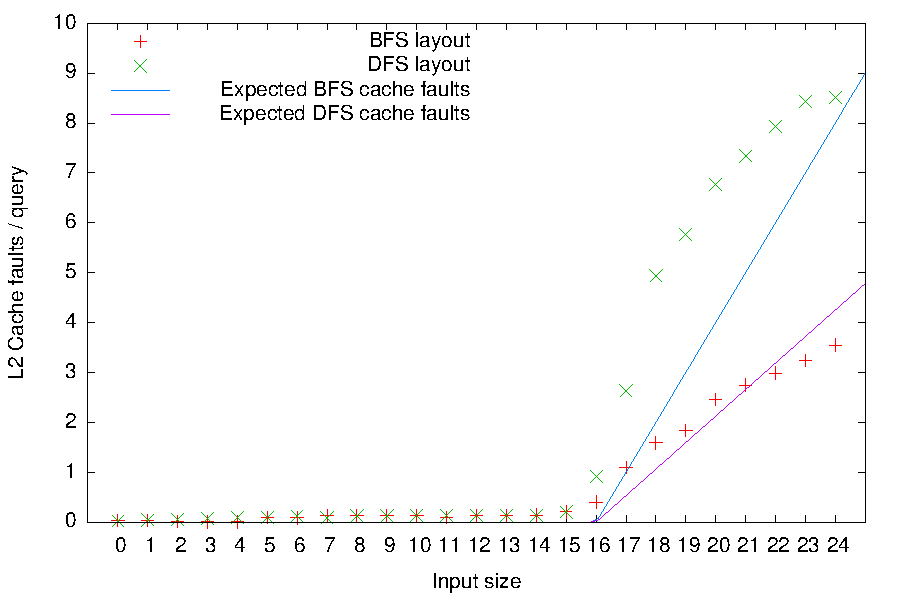
\includegraphics[width=\textwidth]{../week1/plots/outputs/bfs_dfs_cachefaults}
  \caption{L2 cache faults per query of binary DFS and BFS layouts.}
    \label{fig:bfs_dfs_cachefaults}
\end{figure}

\subsection{Blocked BFS layout}

As we have seen in the previous results cache faults play a major role in the performance of the algorithms. Therefore, we decided on testing a blocked BFS layout and various block sizes. We expect fewer cache faults and therefore higher performance.

Figure \ref{fig:blocked_bfs_bs_runningtime} shows that the best performing block sizes are 16 ($d = 17$) and 32 ($d = 33$) when using binary search within the blocks. Our devised formulas indicates that block size 32 should result in slightly more cache faults which figure \ref{fig:blocked_bfs_bs_cachefaults} also shows. The increased number of cache faults is counterbalanced by the number of branch mispredictions which are shown in figure \ref{fig:blocked_bfs_branchmis_runningtime}. The amount of branch mispredictions for block size 32 is slightly lower because at each level we get an extra branch misprediction when the final element is found. And because the height of the tree is lower, we get fewer of those extra mispredictions.

We want to reduce the number of branch mispredictions so instead of using binary search within the block we tried a linear scan. This should make the CPU optimize its pipeline. Figure \ref{fig:blocked_bfs_branchmis_runningtime} shows that linear scan induces fewer branch mispredictions.

The performance when using linear scan is slightly better compared to binary search. Fewer branch mispredictions compensates for the increased number of instructions/comparisons used in linear scan.

\todo{Refs passer ikke}

\begin{figure}[h!]
  \centering
  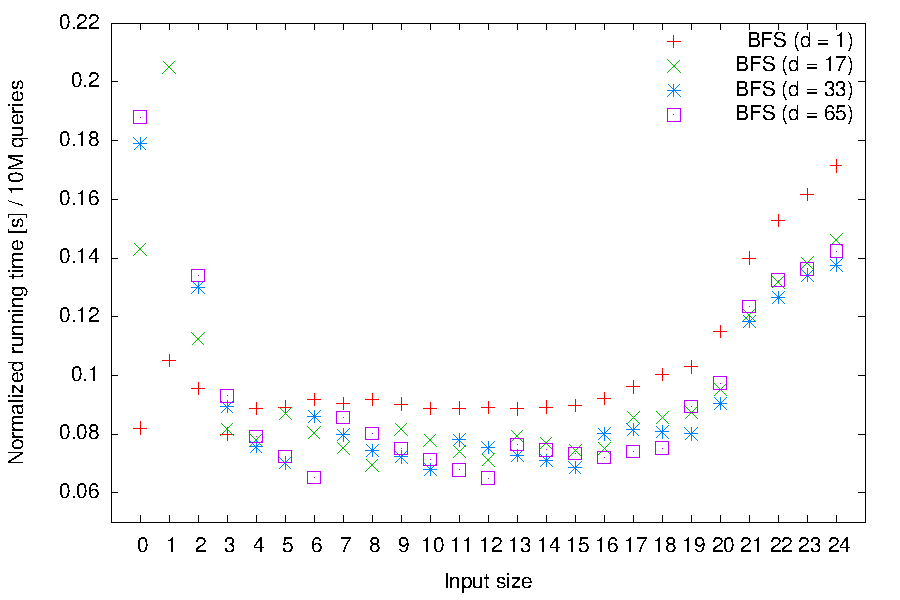
\includegraphics[width=\textwidth]{../week1/plots/outputs/Btree_bs_runningtime}
  \caption{Normalized running time using blocked BFS layout with binary search in each block.}
  \label{fig:blocked_bfs_bs_runningtime}
\end{figure}

\begin{figure}[h!]

  \centering
  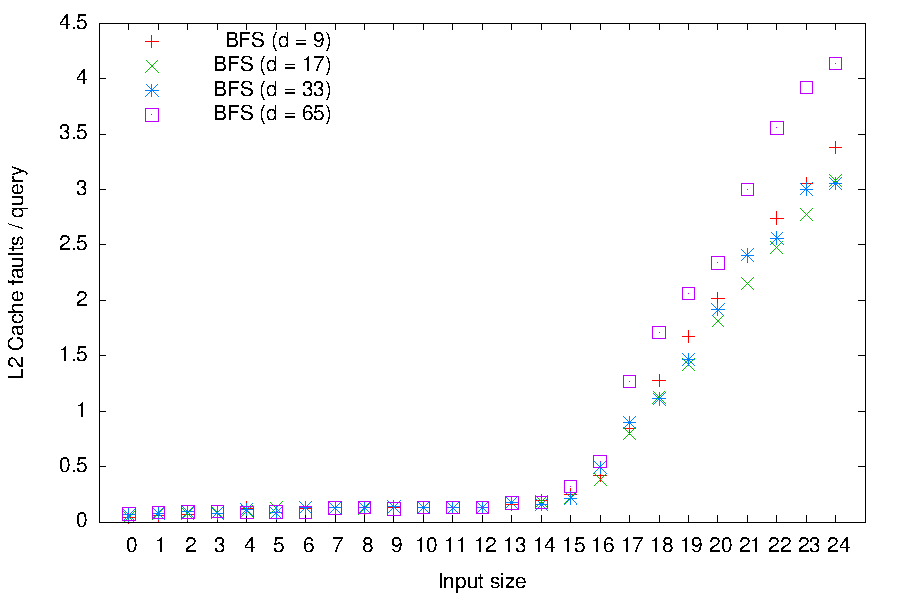
\includegraphics[width=\textwidth]{../week1/plots/outputs/Btree_bs_cachefaults}
  \caption{L2 cache faults per query of using blocked BFS layout with binary search in each block.}
  \label{fig:blocked_bfs_bs_cachefaults}
\end{figure}

\begin{figure}[h!]

  \centering
  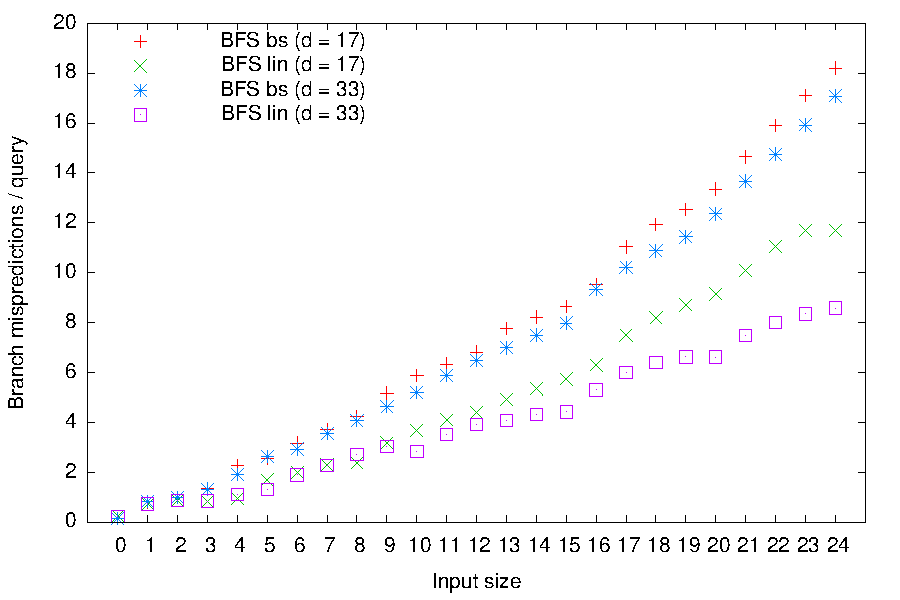
\includegraphics[width=\textwidth]{../week1/plots/outputs/Btree_branchmis}
  \caption{Branch mispredictions in blocked BFS layout using binary search in each block.}
  \label{fig:blocked_bfs_branchmis_runningtime}
\end{figure}

\begin{figure}[h!]

  \centering
  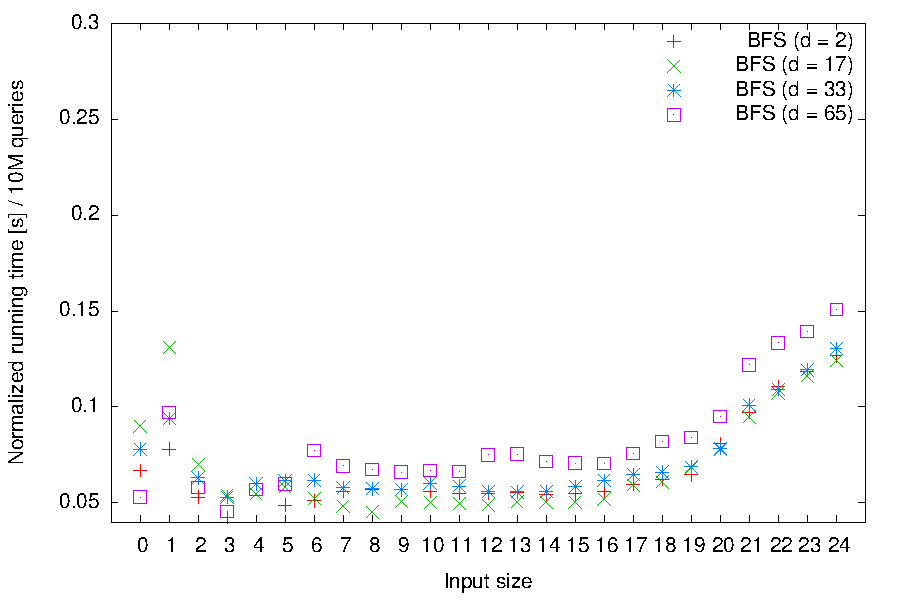
\includegraphics[width=\textwidth]{../week1/plots/outputs/Btree_lin_runningtime}
  \caption{Normalized running time using blocked BFS layout using linear scan in each block.}
  \label{fig:blocked_bfs_lin_runningtime}
\end{figure}

\subsection{Blocked DFS layout}

For binary DFS layout we got more cache faults compared to BFS. This unexpected effect is reduced when the block size is increased. When the block size is 16 and above the effect is diminished completely as shown in \ref{fig:blocked_dfs_lin_runningtime}.

\begin{figure}[h!]
  \centering
  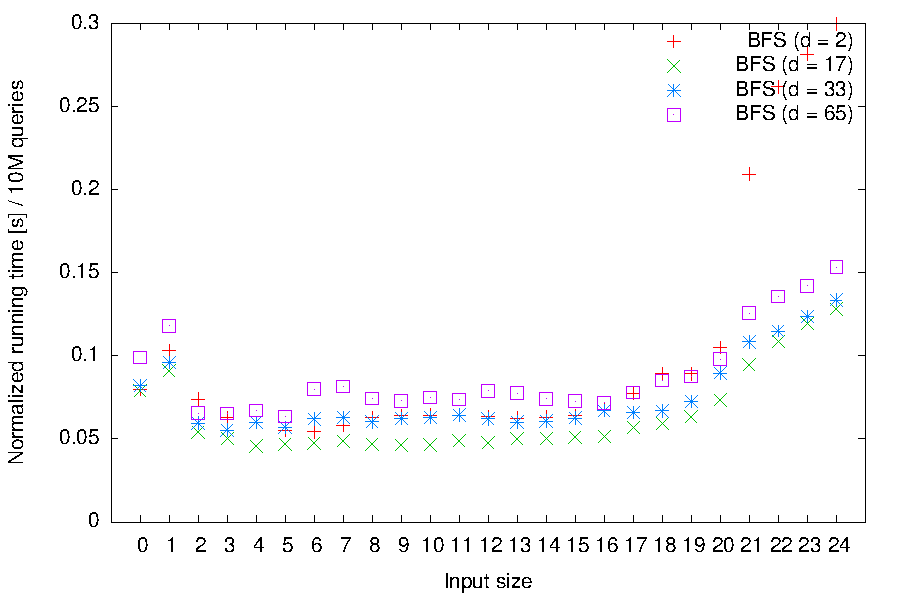
\includegraphics[width=\textwidth]{../week1/plots/outputs/DFS_runningtime}
  \caption{Normalized running time using blocked DFS layout using linear scan in each block.}
  \label{fig:blocked_dfs_lin_runningtime}
\end{figure}

\subsection{Summary}

The best three versions of binary search, BFS and DFS are shown in \ref{fig:champions}. To summarize, blocked linear scan algorithms have the highest throughput and they are far superior to binary search.

\begin{figure}[h!]

  \centering
  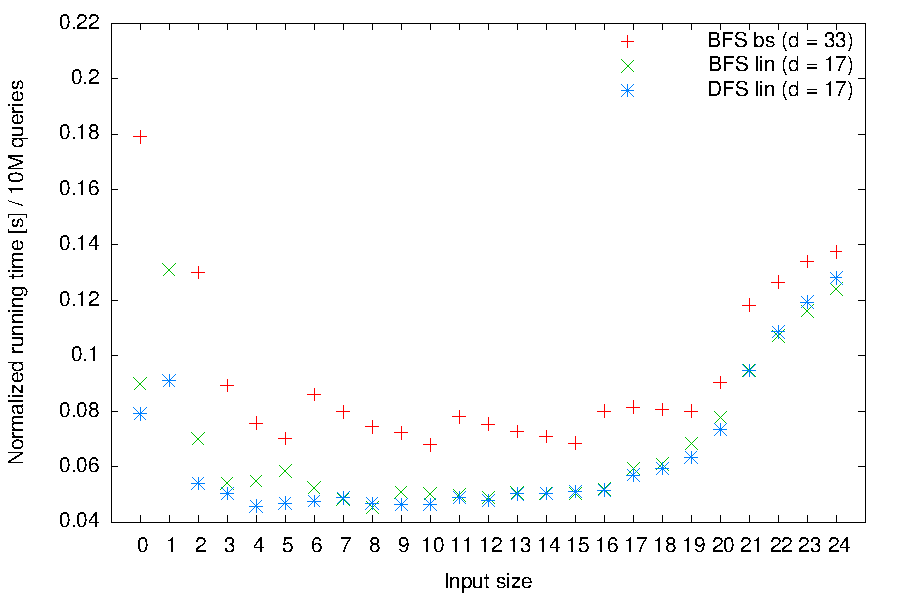
\includegraphics[width=\textwidth]{../week1/plots/outputs/bfs_dfs_16_runningtime}
  \caption{Normalized running time of the best of the three approaches.}
  \label{fig:champions}
\end{figure}
